\begin{center} 
\emph{``Hold fast to dreams\ldots For when dreams go\\ Life is a barren field\ldots Frozen with snow.'' -- Langston Hughes}
\end{center}

\section{Fields}\label{sec:fields}
The topic of this section will be about what is even a number. This discussion is often postponed to more advanced mathematics courses where abstraction is king, but for linear algebra students, this abstraction is just budding. This course will be primarily a computational introduction to linear algebra with select proofs and applications. In spite of this goal, the abstract notion of a field will not hinder this. In fact, the introduction of various fields will strengthen the student's understanding of the concepts and computations of linear algebra as the student will see what parts are truly necessary and when variability is allowed. This will also strengthen the realization that discussion of complex vector spaces and real vector spaces are not two separate discussion but instead one same story.\\

What really is a number? Although numbers are useful for counting, they are much more useful than that.  A simple answer would be to say it is a thing with which we do math on. Although a crude response, this will satisfy our inquiry, thus avoiding a long journey through deep logic and philosophy. Maybe another day.\\

%%%%%%%%%%%%%%%%%%%MOVE TO APPENDIX%%%%%%%%%%%%%%%%%%%%%%%%%%%%%%%%%
A \textbf{set} to us will mean a collection of objects, typically called \textbf{elements}. Those elements could be numbers, colors, people, pok\'{e}mon, or other sets! Typically, sets will be denoted by capital alphabet letters such as $A$, $B$, $C$, etc. and elements with lower case letters such as $a$, $b$, $c$, etc. Typically, $\{\ldots\}$ is used to denote the elements in a set, i.e. $A=\{1, 2, 3, 4\}$. Often a set is described by some rule, such as $A = \{x\mid \text{x satisfies some rule}\}$. If an element $x$ is a member of the set $X$, then we denote this as $x\in A$. Then notation $x\notin A$ means that $x$ is not an element of $A$. There must be a clear rule to decide whether an element is a member of a set or not, otherwise it is not a set. The set which contains no elements, $\emptyset = \{\}$, is called the \textbf{empty set}.\\

A \textbf{function} $f$ is a relationship between sets, say $A$ and $B$, such that each element of $A$ is assigned to exactly one element of $B$ (although not all elements of $B$ must be assigned to an element of $A$). We denote this function relation as $f : A\to B$. If $A$ and $B$ are two sets, we let $A\times B$ denote the set of ordered pairs of elements from $A$ and $B$. For example, if $a\in A$ and $b\in B$, then $(a,b)\in A\times B$. Finally, an \textbf{operation} is a function of the form $f : A\times B \to C$. One should think of an operation as a process of bringing two objects together and creating a third object.\\
%%%%%%%%%%%%%%%%%%%MOVE TO APPENDIX%%%%%%%%%%%%%%%%%%%%%%%%%%%%%%%%%

\subsection{Fields}
 We are now ready for the definition of a field of numbers. Do not panic. If this seems very fast, that is okay. Our discussion will slow down quickly.\\

\begin{Def}\label{def:field} A \textbf{field} is a nonempty set $F$ with elements called \textbf{scalars} on which are defined two operations, called \textbf{addition} $+ : F\times F \to F$ and \textbf{multiplication} $\cdot : F\times F \to F$, such that for all scalars $a, b, c \in F$, the following ten axioms hold:
\setlength{\columnsep}{30pt}
\begin{multicols}{2}
\begin{enumerate}[label=\emph{(\roman*)}, series=!DEF!]
\item\label{ax:addcom} $a+b=b+a$ 
\item\label{ax:addass} $(a+b)+c=a+(b+c)$ 
\item\label{ax:addid} There exists  a scalar $0\in F$, such that\\ $a + 0 = 0 + a = a$ 
\item\label{ax:addinv} For each $a$, there exists a scalar $-a \in F$, such that $a + (-a) = (-a) + a = 0$ 
\item $a\cdot (b+c) = (a b) + (a c)$\columnbreak
\item\label{ax:multcom} $ab=b a$ 
\item\label{ax:multass} $(a b)c=a(b c)$ 
\item\label{ax:multid} There exists  a scalar $1\in F$, such that\\ $a  1 = 1  a = a$ 
\item\label{ax:multinv} For each $a\neq 0$, there exists a scalar $a^{-1} \in F$, such that $a  a^{-1} = a^{-1}  a = 1$ 
\item $(a+b)\cdot c = (a c) + (b c)$
\end{enumerate}
\end{multicols}
\end{Def}

It might seem like a daunting list but remember the following: a field is just a number system for which we can add, subtract, multiply, and divide following the usual commutative, associative, and distributive laws. The set of rational numbers, denoted $\Q$, is a field. The set of real numbers $\R$ and the set of complex numbers $\C$ are also both fields. These are the fields that we are most familiar with. Note that the set of integers $\Z$ is NOT a field, as the quotient of two integers is not always an integer, e.g. $\dfrac{1}{2}\notin \Z$. Likewise, the set of natural numbers $\N$ is NOT a field for the same reasons with division but also because the difference of two natural numbers is not always a natural number, e.g. $3-4 = -1 \notin \N$.\\

Fields are the number systems we are used to in previous algebra classes. For example, fields are exactly the environment where linear equations can be solved. Let $F$ be a field and $ax+b=c$ is a linear equation\label{note:lineareqn} with variable $x$ and $a,b,c\in F$. Here the variable itself is a placeholder for some other scalar. A \textbf{solution} to this linear equation is an assignment to the variable $x$ which makes the equation true. For linear equations, we see there is only one solution in any field:
\begin{align*}
ax+b&=c&\\
(ax+b)+(-b)&=c+(-b)& \text{Existence of Additive Inverses \eqref{ax:addinv}}\\
ax+(b-b)&=c-b& \text{Additive Associativity \eqref{ax:addass}}\\
ax+0&=c-b& \\
ax&=c-b& \text{Existence of Additive Identity \eqref{ax:addid}}\\
a^{-1}(ax)&=a^{-1}(c-b)& \text{Existence of Multiplicative Inverses \eqref{ax:multinv}}\\
(a^{-1}a)x&=\dfrac{c-b}{a}& \text{Multicative Associativity \eqref{ax:multass}}\\
1x&=\dfrac{c-b}{a}& \\
x&=\dfrac{c-b}{a}& \text{Existence of Multicative Identity \eqref{ax:multid}}\\
\end{align*}

Note that commutativity is used to guarantee that subtraction and division is well-defined. Therefore, a linear equation has a unique solution over a field.\\

\begin{Exam} Solve the following equations:
\begin{enumerate}
\item $2x+1=6$ over $\Q$\\
\[2x+1=6 \qRightarrow 2x = 6-1=5 \qRightarrow x = \fbox{$\dfrac{5}{2}$}.\]

\item $(i+1)x + (3-i) = 4+5i$ over $\C$\\
\[ (i+1)x + (3-i) = 4+5i \qRightarrow (i+1)x = (4+5i) - (3-i) = 1+6i\]\[ \qRightarrow x = \dfrac{1+6i}{1+i} = \dfrac{1+6i}{1+i}\left(\dfrac{1-i}{1-i}\right) = \dfrac{1-i+6i+6}{1-i+i+1} = \fbox{$\dfrac{7}{2} + \dfrac{5}{2}i$}.\qedhere\]
\end{enumerate}
\end{Exam}\vs


\subsection{Modular Arithmetic and Finite Fields}
We introduce now one last type of field: a finite field. Let $n$ be a positive integer and let $a$ be any integer. Consider the operation $a\div n$. The division algorithm known unto us since primary school guarantees there are unique integers $q, r$, called the \emph{quotient} and \emph{remainder}, respectively, such that $a=qn+r$ where $0\le r< n$. For example, for $n=5$ and $a=13$, we have that $13=2(5) + 3$, that is, $q=2$ and $r=3$. We generally would interpret this statement as $5$ divides into $13$ two times with remainder of three, that is, if $13$ vectors are to be shared among $5$ friends then each friend would get $2$ vectors with $3$ vectors left over. Typically, with a division problem one is interested in finding the quotient but in \textbf{modular arithmetic}, one is instead interested in finding the remainder, which has many powerful uses. Let $\Z_n = \{0, 1, 2, \ldots, n-1\}$. Then $\Z_n$ should be viewed as the set of all possible remainders, or \textbf{residues}, when divided by $n$. Define next a function $\pmod n : \Z \to \Z_n$ by the rule $a \pmod n$ is the unique remainder of $a$ when divided by $n$. For example, $8 \pmod 5 = 3$. Likewise, $14\pmod 5 = 4$ since $14=2(5)+4$, that is, $5$ divides into $14$ twice with a remainder of $4$. The residue $a\pmod n$ is read "$a$ modulo $n$" and $n$ is called \textbf{modulus} of the function.\\

Note that if $0\le a < n$, then $a\pmod n = a$, the original value, for example, $3\pmod 5 = 3$. In this example, the associated quotient is $0$. This is a department from decimal division where the fraction $\frac{3}{5}$ may be expressed as the decimal $0.6$. Special attention should also be given to when $a$ is a negative integer. Note that $-11 \pmod 6 = 1$ since $-11 = (-2)(6) + 1$, where the quotient is $-2$ and the residue is $1$. This is in contrast to the possibility $-11 = (-1)(6) + (-5)$. The difference here is that while quotients may be any integer: positive, zero, or negative, remainder must always exist in the range $0\le r \le n-1$, which is necessarily nonnegative. \\

When $a\ge n$, one way to determine $a\pmod n$ is to subtract from $a$ the modulus $n$ until the difference lies in $\Z_n$. For example, $14>5$, the first difference $14-(1)5 =14-5=  9$ is still too large. The second difference $14-2(5) = 9-5 = 4\in \Z_5$. Thus, $14\pmod 5=4$, as observed above. This notion of repeated subtraction is actually where the division algorithm gets its life, in a similar way of viewing multiplication as repeated addition. When $a$ is negative, we can instead add the modulus $n$ to $a$ (or subtract a negative, if one prefers) until the sum lies inside of $\Z_n$. For examples, $-11-(-1)6=-11+6= -5$ which is too small, but the next iteration $-11-(-2)6 = -5+6 = 1$. Thus, $-11\pmod 6=1$, as observed above. \\

Note that $7\pmod 6 = 1 = -11 \pmod 6$, that is, it is possible for two different integers to have the same remainder when divided by the modulus $n$. We say that two integers $a$ and $b$ are \textbf{congruent modulo}\label{def:modularcongruence} $n$ if $a\pmod n = b\pmod n$ and denote this congruence as $a\equiv b \pmod n$. For example, $7\equiv 12 \pmod 5$ since $7$ and $12$ both have remainder 2. If $a\equiv b \pmod n$, then $a=q_1n + r$ and $b=q_2n+r$ for some quotients $q_1, q_2$. Then their difference $a-b = (q_1-q_2)n$ is a multiple of the modulus $n$. In other words, $a\equiv b \pmod n$ if and only if $a-b$ is divisible by $n$. For example, $12-7=5$ which implies that $12\equiv 7\pmod 5$.\\

 We define two operations on $\Z_n$ called \textbf{modular addition} and \textbf{modular multiplication}: modular addition is defined by the rule that two integers are added together and the sum's remainder modulo $n$ is reported, modular multiplication is defined similarly. The final result should be a number in $\Z_n$.\\

A visual interpretation of modular addition would be the following. Imagine $n$ pearls on a string labeled from left to right with the numbers $0$ through $n-1$. Take the two ends of this string and connect them together to form a pearl necklace of integers. To compute $a+b \pmod n$, start at the pearl labeled $a$ and rotate the necklace by one pearl to the right (counter-clockwise) exactly $b$ times. The pearl you land on is then modular sum of $a$ and $b$. For example, starting at $2$ and counting forward on necklace with $5$ pearls $4$ times gives the pearl $1$, that is, $2+4\equiv 1\pmod 5$.  Modular multiplication can similarly be visualized as iterated addition on the pearl necklace.\\

\centerline{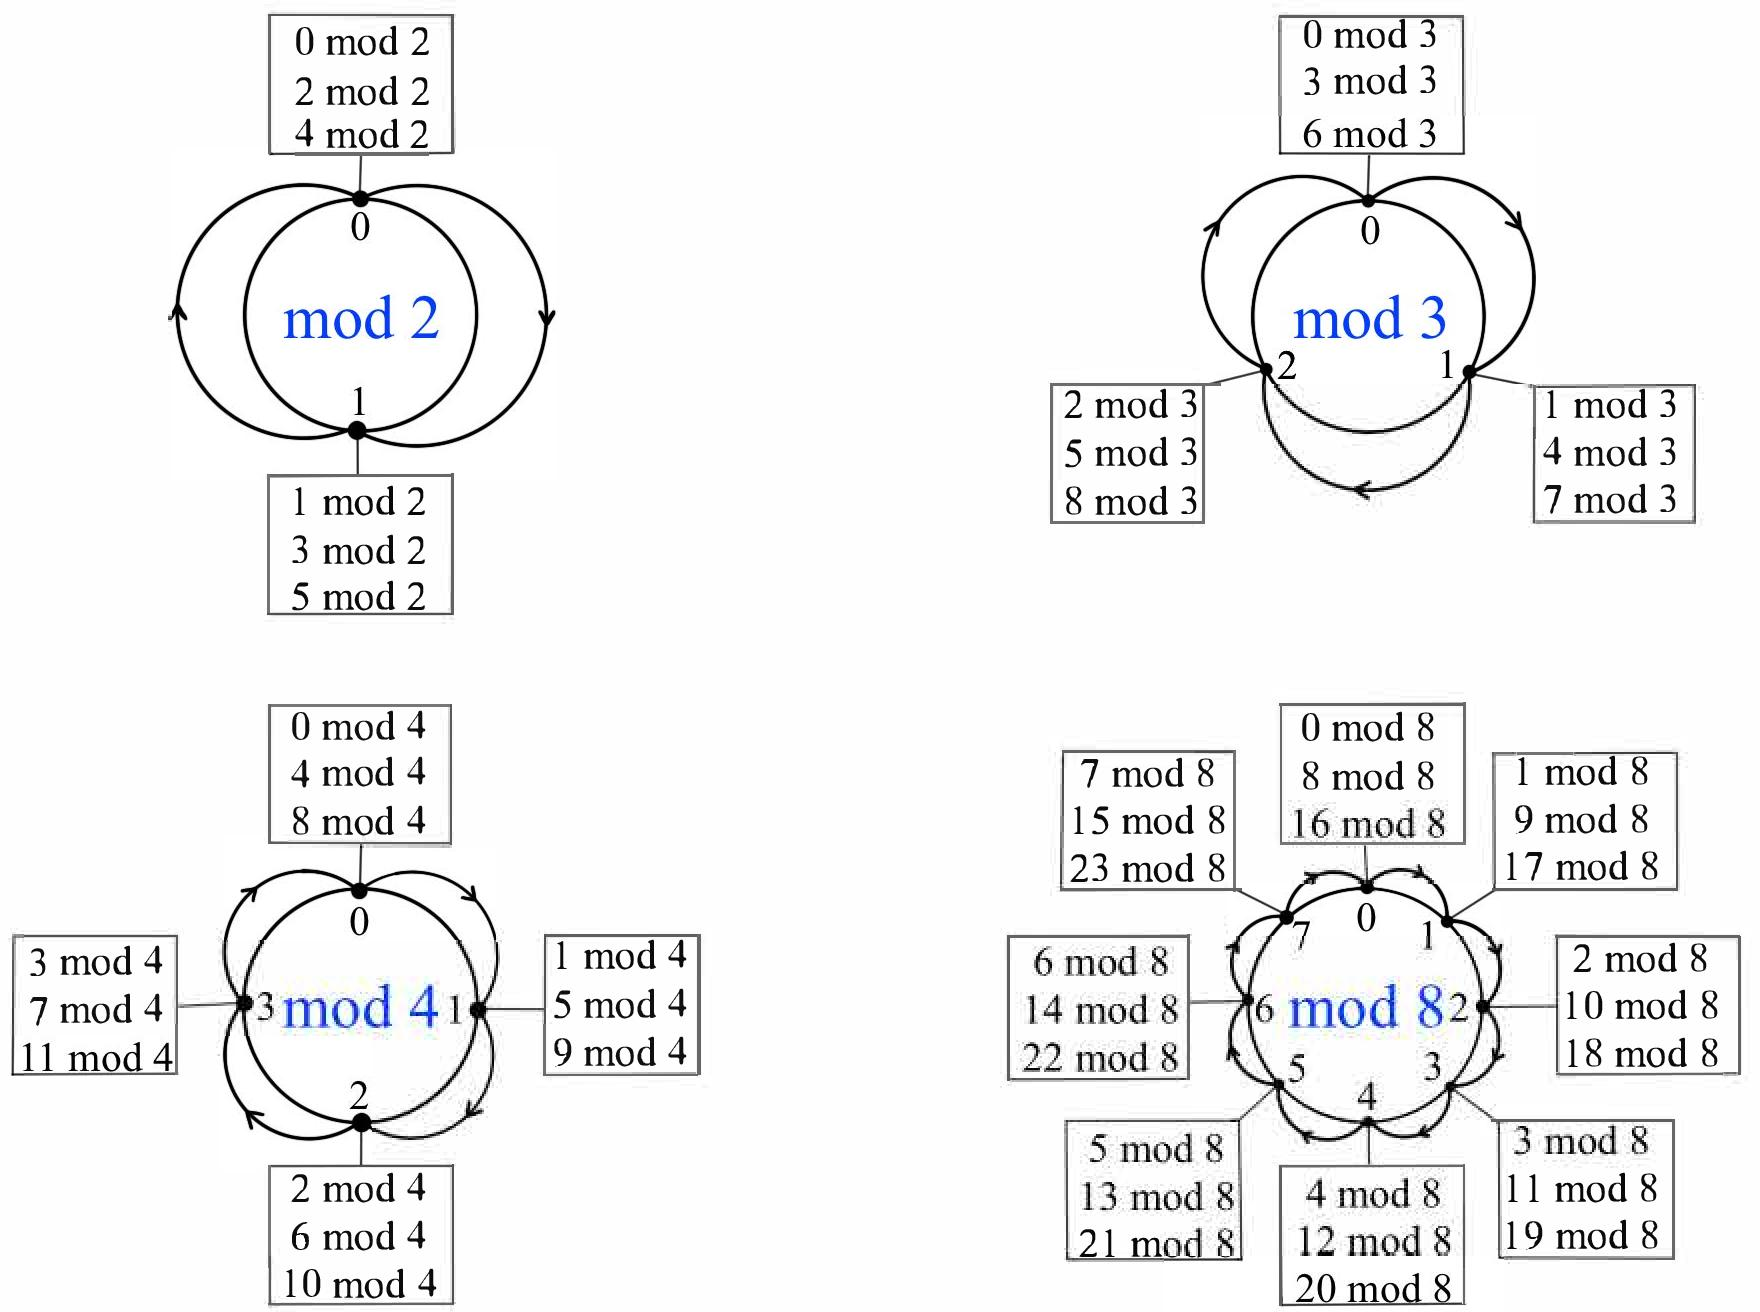
\includegraphics[scale=1]{Chapter1/images/necklace.png}} %Adym Warhurst

\begin{Exam}\label{exam:1.2modcalc} Let consider the following calculations: 
\begin{enumerate}
\item $6+11 \pmod 5$\\
\[6+11\equiv 17\equiv \fbox{$2$} \pmod 5\]
\item $7+13 \pmod 5$\\
\[7+13 \equiv 20\equiv \fbox{$0$} \pmod 5\]
\item\label{item:1.2inverse} $2(4) \pmod{7}$\\
\[2(4) \equiv 8\equiv 1 \pmod 7.\]
\item $2(5+6) \pmod{13}$\\
\[ 2(5+6) \equiv 2(11) \equiv 22 \equiv \fbox{$9$} \pmod{13}\]
\item $3(5)+8 \pmod{11}$\\
\[3(5)+8 \equiv 15+8 \equiv 4+8 \equiv 12 \equiv \fbox{$1$} \pmod{11}\qedhere\]
\end{enumerate}
\end{Exam}\vs

We can define \textbf{modular subtraction} $a-b \pmod n$ by adding the additive inverse of $b$ with respect to modular addition, that is, $a-b \equiv a+(-b)\pmod n$. Thus, modular subtraction is the inverse operation of modular addition. Returning to the pearl necklace analogy above, if $a+b\pmod n$ turns the necklace to the right (counter-clockwise) $b$ times from $a$, $a-b\pmod n$ turns the necklace to the left (clockwise) $b$ times from $a$. For example, starting at $2$ and counting backward on the necklace with $5$ pearls $4$ times gives the pearl $3$, that is, $2-4\equiv 3\pmod 5$. Likewise, $14-5 \equiv 9 \equiv 1\pmod 8$. %(Brittany Palmer)
Note that $-b \equiv n-b \pmod n$. Thus, the final result when computing modular subtraction should always be positive.\\ %Example by Zach Rogers

Similarly, we define  \textbf{modular division} $a/b \pmod n$ by multiplying by the multiplicative inverse of $b$ with respect to modular multiplication, that is, $a/b \equiv ab^{-1} \pmod n$. This multiplicative inverse will be an element of $\Z_n$ such that $bb^{-1} \equiv 1 \pmod n$, that is, their product will be one more than a multiple of $n$ as this implies the remainder is $1$ when divided by $n$ (see Example \ref{exam:1.2modcalc}.\ref{item:1.2inverse}). For example, \[4^{-1} = \dfrac{1}{4}\equiv 2 \pmod 7\] since $4(2) = 8 \equiv 1\pmod 7$. Thus, \[\dfrac{5}{4} \equiv 5(2) = 10 \equiv 3\pmod 7.\]  This multiplicative inverse does not always exists (see Exercise \ref{ex:1.2nosoln}).\\ %Example by Zach Rogers

 Alternatively, one can simplify a modular fraction without a multiplicative inverse by replacing the numerator with an integer equivalent to the original but actually divisible by the denominator in the usual sense. For example, \[\dfrac{17}{3} \equiv \dfrac{17+10}{3} \equiv \dfrac{27}{3} \equiv \dfrac{9(3)}{3} \equiv 9\pmod 5.\] The following theorem characterizes when this can be done.\\

\begin{Thm} The set $\Z_n$ is a field with respect to modular addition and modular multiplication if and only if $n$ is a prime number.
\end{Thm}\vs

\begin{Exam} Solve the linear equation $2x+1\equiv 6 \pmod{13}$. \\ 

Since $\Z_{13}$ is a field, we can solve this linear equation in the same fashion as the previous ones. Note
\[2x+1\equiv 6 \qRightarrow 2x \equiv 6-1 \equiv 5 \pmod {13} \qRightarrow x \equiv \dfrac{5}{2} \equiv 5(2)^{-1}.\] Next, we need to either identify the reciprocal of $2 \pmod{13}$\footnotemark[2] or replace $5$ with a congruent integer which is even, that is, $\dfrac{5}{2} \equiv \dfrac{5+13}{2} \equiv \dfrac{18}{2} \equiv 9\pmod{13}$. Therefore, the solution is 9. We can check this solution:
\[2(9) +1 \equiv 18 + 1 \equiv 19 \equiv 6 \pmod{13}.\qedhere\]
\end{Exam}\vs 

\begin{Exam} Solve the linear equation $3x+5\equiv 1 \pmod{7}$. \\ %Luke Shaner

We solve this equation similar to the previous example over the field $\Z_{7}$. 
\[3x+5\equiv 1 \qRightarrow 3x \equiv 1-5 \equiv -4 \equiv 3 \pmod {7} \qRightarrow x \equiv \dfrac{3}{3} \equiv 1.\]  We can check this solution:
\[3(1)+5 \equiv 3+5 \equiv 8 \equiv 1 \pmod{7}.\qedhere\]
\end{Exam}\vs
 
%%%%%%%%%%%%%%%%%%% Exercises %%%%%%%%%%%%%%%%%%%
\startExercises{fields}

\begin{enumerate}[!HW!, start=1]
\item Explain the difference between equality of \hyperref[note:integers]{integers} and \hyperref[def:modularcongruence]{congruence modulo $p$}. %Adam Maxwell
\end{enumerate}

\noindent For Exercises \ref{true:fieldsstart}-\ref{true:fieldsstop}, determine with the statement is true or false. If false, correct the statement so that it is true.
\begin{enumerate}[!HW!]
\item\label{true:fieldsstart} The remainder $a\pmod n$ is read ``$a$ modulo $n$'' and $a$ is called the modulus of \hyperref[note:mod]{$\Z_n$}. %Carson Blickenstaff
\item It is possible for two different integers to have the same residue modulo $n$. %Carson Blickenstaff
\item Modular division $a/b\pmod n$ is defined by multiplying by the inverse of $b$ with respect to modular addition. %Carson Blickenstaff
\item The set $\Z_n$ is a field with respect to modular addition and multiplication if and only if $n$ is a real number. %Carson Blickenstaff
\item\label{true:fieldsstop} If $0\le a< n$, then $a\pmod n=n$.\\ %Carson Blickenstaff
\end{enumerate}

\noindent For Exercises \ref{exer:modsimplifystart}-\ref{exer:modsimplifystop}, simplify the \hyperref[exam:1.2modcalc]{modular expression}. 
\begin{enumerate}[!HW!]
\begin{multicols}{4}
\item\label{exer:modsimplifystart} $-4\pmod{7}$ %Hamza Samha
\item $-21\pmod{5}$ %Hamza Samha
\item $-1076 \pmod{4}$ %Hamza Samha
\item $-686 \pmod{13}$ %Hamza Samha
\end{multicols}
\begin{multicols}{4}
\item $2237 \pmod{11}$ %Jaden Torgerson
\item $\dfrac{1}{2} \mod 3$ %Morganne Skelton
\item $\dfrac{1}{3} \mod 7$ %Morganne Skelton
\itemspade $34 + 61 \pmod{7}$
\end{multicols}
\begin{multicols}{3}
\itemspade $4(13) \pmod 5$
\item $5(15)\pmod 6$ %Yinglong Niu
\item $2(8-5) +4 \pmod 3$ %Yinglong Niu
\end{multicols}
\begin{multicols}{2}
\itemspade $2(6-3)+7 \pmod 2$
\itemspade $3[2+1-(6+3)] +6(7) \pmod{13}$
\end{multicols}
\begin{multicols}{3}
\itemspade $\dfrac{5(4)+3}{2(6)} \pmod{7}$
\item $\dfrac{3(5)+4}{2(7)} \pmod 9$ %Yinglong Niu
\item $\dfrac{6(7)+5}{2(4)} \pmod{13}$ %Heming Zu
\end{multicols}
\begin{multicols}{2}
\item $2[(3+4+2+5)+1+2(3)-3+2(-2)] \pmod 7$ %Mattie Zeigler
\item\label{exer:modsimplifystop} $\dfrac{4(9)+1-(6+12)}{1+3(6)} \pmod{13}$ %Mattie Zeigler
\end{multicols}
\item $\dfrac{-2(35-74)}{3} \pmod{19}$ %Sarah Walters
\end{enumerate}\vs

\noindent For Exercises \ref{exer:fieldequationRealstart}--\ref{exer:fieldequationRealstop}, solve the \hyperref[note:lineareqn]{linear equation}.  
\begin{enumerate}[!HW!]
\begin{multicols}{3}
\item\label{exer:fieldequationRealstart} $7x+10=3$ %Jaxton Maez
\itemspade $6x+7=2$
\itemspade $(2+i)x + (5-7i) = 3-4i$
\end{multicols}
\begin{multicols}{3}
\item $3x+7\equiv 5 \pmod 5$ %Kaylee Hall
\itemspade $x+1\equiv 0 \pmod 2$ 
\itemspade $2x+3\equiv 4 \pmod 5$ 
\end{multicols}
\begin{multicols}{3}
\itemspade $3x+2\equiv 1 \pmod 7$ 
\itemspade $5x+1\equiv 4 \pmod{11}$ 
\item $420x-7\equiv 98 \pmod{11}$  %Jaden Torgerson
\end{multicols}
\begin{multicols}{3}
\item $2x+5\equiv 0 \pmod 7$ %anon
\item $14x+12\equiv 124\pmod 6$ %Courtney Flanigan
\item $5x-25\equiv 71\pmod{14}$ %Courtney Flanigan
\end{multicols}
\begin{multicols}{3}
\item $2x-4\equiv 14\pmod 7$ %Courtney Flanigan
\item $3(2-4(x+1))\equiv 27\pmod 3$ %Courtney Flanigan
\item $-20-4x\equiv 40\pmod 4$ %Courtney Flanigan
\end{multicols}
\begin{multicols}{3}
\item $5x+22\equiv 15 \pmod 8$ %Grayson Walker
\item $6x+\frac{5}{2} \equiv 0 \pmod 7$ %Da Huo
\item\label{exer:fieldequationRealstop} $(3+10)x+2(7)+3\equiv 5(14) \pmod 7$ %anon
\end{multicols}
\end{enumerate}

\begin{enumerate}[!HW!]
\itemspade\label{ex:1.2nosoln} Show that the \hyperref[note:lineareqn]{linear equation} $2x+3\equiv 4 \pmod 6$ has no solution. 
\end{enumerate}

%%%%%%%%%%%%%%%%%%% Footnotes %%%%%%%%%%%%%%%%%%%
\mbox{}\vfill

\footnotetext[2]{By the way, the reciprocal of $2$ modulo $13$ is $7$ since $2(7) \equiv14\equiv 1 \pmod{13}$. Note that $x\equiv 5(2)^{-1} \equiv 5(7) \equiv 35 \equiv 9 \pmod{13}$.}
\pagebreak